\documentclass[12pt]{article}
\usepackage[margin=2.5cm]{geometry}
\usepackage{enumerate}
\usepackage{amsfonts}
\usepackage{amsmath}
\usepackage{fancyhdr}
\usepackage{amsmath}
\usepackage{amssymb}
\usepackage{amsthm}
\usepackage{mdframed}
\usepackage{graphicx}
\usepackage{subcaption}
\usepackage{adjustbox}
\usepackage{listings}
\usepackage{xcolor}
\usepackage{booktabs}
\usepackage[utf]{kotex}
\usepackage{hyperref}

\definecolor{codegreen}{rgb}{0,0.6,0}
\definecolor{codegray}{rgb}{0.5,0.5,0.5}
\definecolor{codepurple}{rgb}{0.58,0,0.82}
\definecolor{backcolour}{rgb}{0.95,0.95,0.92}

\lstdefinestyle{mystyle}{
    backgroundcolor=\color{backcolour},
    commentstyle=\color{codegreen},
    keywordstyle=\color{magenta},
    numberstyle=\tiny\color{codegray},
    stringstyle=\color{codepurple},
    basicstyle=\ttfamily\footnotesize,
    breakatwhitespace=false,
    breaklines=true,
    captionpos=b,
    keepspaces=true,
    numbers=left,
    numbersep=5pt,
    showspaces=false,
    showstringspaces=false,
    showtabs=false,
    tabsize=1
}

\lstset{style=mystyle}

\pagestyle{fancy}
\renewcommand{\headrulewidth}{0.4pt}
\lhead{Team Treehouse}
\rhead{Modifying Data with SQL Part 3 Notes}

\begin{document}
\title{Modifying Data with SQL Part 3 Notes}
\author{Team Treehouse}
\maketitle

\bigskip

\section{Removing Data from All Rows in a Table}

\bigskip

\begin{itemize}
    \item \textbf{Syntax:} DELETE FROM \textit{table name};
    \item deletes all data in a table
    \item doesn't remove table

    \bigskip

    \underline{\textbf{Example:}}

    \bigskip

    \begin{lstlisting}[language=SQL]
    DELETE FROM logs;
    DELETE FROM users;
    DELETE FROM products;
    \end{lstlisting}
\end{itemize}

\bigskip

\section{Removing Specific Rows}

\bigskip


\begin{itemize}
    \item \textbf{Syntax:} DELETE FROM \textit{table name} WHERE \textit{condition};

    \bigskip

    \underline{\textbf{Example:}}

    \bigskip

    \begin{lstlisting}[language=SQL]
    DELETE FROM users WHERE email = "andrew@teamtreehouse.com";
    DELETE FROM movies WHERE genre = "Musical";
    DELETE FROM products WHERE stock_count = 0;
    \end{lstlisting}

\end{itemize}


\bigskip

\section{Review and Practice}

\bigskip

\section{Quiz 1}

\bigskip

\begin{enumerate}[1.]
    \item

    What keyword would you use to remove rows from a table?

    \bigskip

    \begin{enumerate}[A.]
        \item REMOVE
        \item DELETE
        \item UPDATE
    \end{enumerate}

    \bigskip

    \textbf{Answer:} B

    \item

    \begin{center}
    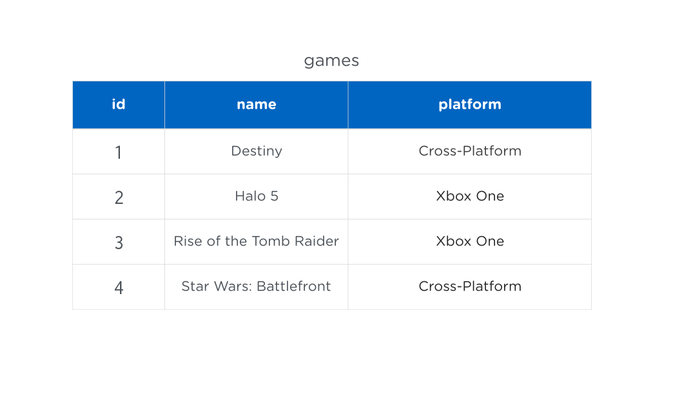
\includegraphics[width=0.8 \linewidth]{images/part_3_notes_1.png}
    \end{center}

    \bigskip

    What will be left in this table with this DELETE statement?

    \bigskip

    \begin{lstlisting}[language=SQL]
    DELETE FROM games;
    \end{lstlisting}

    \bigskip

    \begin{enumerate}[A.]
        \item Nothing. Everything is deleted.
        \item Only Xbox games.
        \item Only Cross-Platform games.
    \end{enumerate}

    \bigskip

    \textbf{Answer:} A

    \item

    Please fill in the correct answer in each blank provided below.

    \bigskip

    \begin{lstlisting}[language=SQL]
    DELETE FROM cereals \_\_\_ name = "Frosted Flakes";
    \end{lstlisting}

    \bigskip

    \textbf{Answer:} WHERE

    \item

    Which keywords are used for creating rows in a table?

    \bigskip

    \begin{enumerate}[A.]
        \item CREATE INTO
        \item INSERT ROW
        \item CREATE ROW
        \item INSERT INTO
    \end{enumerate}

    \bigskip

    \textbf{Answer:} D

\end{enumerate}


\end{document}